%%%%%%%%%%%%%%%%%%%%%%%%%%%%%%%%%%%%%%%%%
% Stylish Article
% LaTeX Template
% Version 1.0 (31/1/13)
%
% This template has been downloaded from:
% http://www.LaTeXTemplates.com
%
% Original author:
% Mathias Legrand (legrand.mathias@gmail.com)
%
% License:
% CC BY-NC-SA 3.0 (http://creativecommons.org/licenses/by-nc-sa/3.0/)
%
%%%%%%%%%%%%%%%%%%%%%%%%%%%%%%%%%%%%%%%%%

%----------------------------------------------------------------------------------------
%	PACKAGES AND OTHER DOCUMENT CONFIGURATIONS
%----------------------------------------------------------------------------------------

\documentclass[fleqn,10pt]{SelfArx} % Document font size and equations flushed left

\setlength{\columnsep}{0.55cm} % Distance between the two columns of text
\setlength{\fboxrule}{0.75pt} % Width of the border around the abstract

\definecolor{color1}{RGB}{0,0,90} % Color of the article title and sections
\definecolor{color2}{RGB}{0,20,20} % Color of the boxes behind the abstract and headings

\newlength{\tocsep} 
\setlength\tocsep{1.5pc} % Sets the indentation of the sections in the table of contents
\setcounter{tocdepth}{3} % Show only three levels in the table of contents section: sections, subsections and subsubsections

\usepackage{lipsum} % Required to insert dummy text

\usepackage{tikz}
\usetikzlibrary{automata,positioning,fit}

%----------------------------------------------------------------------------------------
%	ARTICLE INFORMATION
%----------------------------------------------------------------------------------------

\JournalInfo{Working Paper} % Journal information
\Archive{} % Additional notes (e.g. copyright, DOI, review/research article)

\PaperTitle{Tikz snippet for drawing ANN diagrams} % Article title

\Authors{Alexandre Trilla\textsuperscript{1}*} % Authors
\affiliation{\textsuperscript{1}\textit{Research Engineer, http://atrilla.net}} % Author affiliation
\affiliation{*\textbf{Corresponding author}: alex@atrilla.net} % Corresponding author

\Keywords{Artificial Neural Network} % Keywords - if you don't want any simply remove all the text between the curly brackets
\newcommand{\keywordname}{Keywords} % Defines the keywords heading name

\Abstract{ANN diagrams.}

%----------------------------------------------------------------------------------------

\begin{document}

\flushbottom % Makes all text pages the same height

\maketitle % Print the title and abstract box

%\tableofcontents % Print the contents section

\thispagestyle{empty} % Removes page numbering from the first page

%----------------------------------------------------------------------------------------
%	ARTICLE CONTENTS
%----------------------------------------------------------------------------------------

\begin{figure*}[!h]\centering % Using \begin{figure*} makes the figure take up the entire width of the page
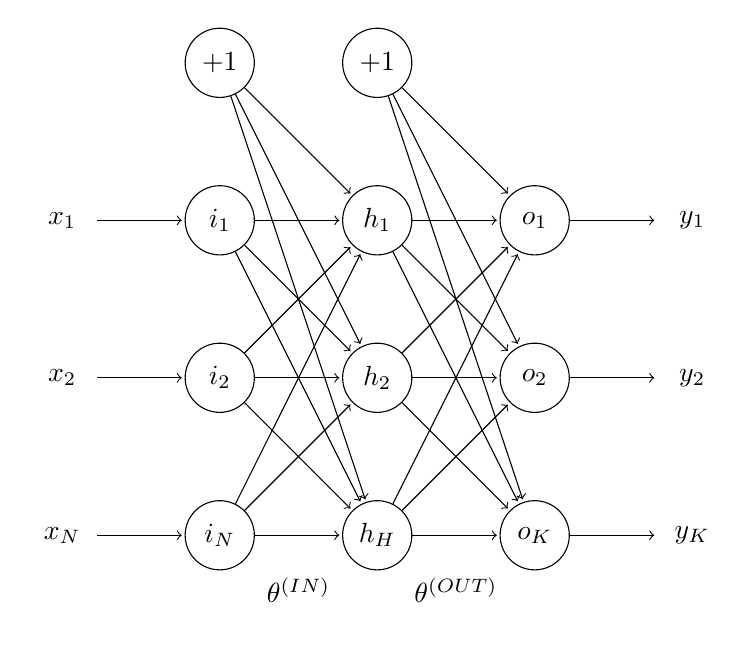
\begin{tikzpicture}[shorten >=1pt,on grid,auto,node distance=2cm] 
   \node[state] (x1)  [draw=none]  {$x_1$}; 
   \node[state] (x2)   [draw=none,below=of x1] {$x_2$}; 
   \node[state] (xN)   [draw=none,below=of x2] {$x_N$}; 
   \node[state] (i1)   [right=of x1] {$i_1$}; 
   \node[state] (ione)   [above=of i1] {+1}; 
   \node[state] (i2)   [below=of i1] {$i_2$}; 
   \node[state] (iN)   [below=of i2] {$i_N$}; 
   \node[state] (hone)   [right=of ione] {+1}; 
   \node[state] (h1)   [below=of hone] {$h_1$}; 
   \node[state] (h2)   [below=of h1] {$h_2$}; 
   \node[state] (hH)   [below=of h2] {$h_H$}; 
   \node[state] (o1)   [right=of h1] {$o_1$}; 
   \node[state] (o2)   [below=of o1] {$o_2$}; 
   \node[state] (oK)   [below=of o2] {$o_K$}; 
   \node[state] (y1)   [draw=none,right=of o1] {$y_1$}; 
   \node[state] (y2)   [draw=none,below=of y1] {$y_2$}; 
   \node[state] (yK)   [draw=none,below=of y2] {$y_K$}; 
   \path[->] 
        (x1) edge node {} (i1)
        (x2) edge node {} (i2)
        (xN) edge node {} (iN)
        (ione) edge node {} (h1)
        (ione) edge node {} (h2)
        (ione) edge node {} (hH)
        (i1) edge node {} (h1)
        (i1) edge node {} (h2)
        (i1) edge node {} (hH)
        (i2) edge node {} (h1)
        (i2) edge node {} (h2)
        (i2) edge node {} (hH)
        (iN) edge node {} (h1)
        (iN) edge node {} (h2)
        (iN) edge node [below] {$\begin{array}{c}\\\theta^{(IN)}\end{array}$} (hH)
        (hone) edge node {} (o1)
        (hone) edge node {} (o2)
        (hone) edge node {} (oK)
        (h1) edge node {} (o1)
        (h1) edge node {} (o2)
        (h1) edge node {} (oK)
        (h2) edge node {} (o1)
        (h2) edge node {} (o2)
        (h2) edge node {} (oK)
        (hH) edge node {} (o1)
        (hH) edge node {} (o2)
        (hH) edge node [below] {$\begin{array}{c}\\\theta^{(OUT)}\end{array}$} (oK)
        (o1) edge node {} (y1)
        (o2) edge node {} (y2)
        (oK) edge node {} (yK)
        ;
\end{tikzpicture}
\caption{Multilayer Perceptron}
\end{figure*}



\begin{figure*}[!h]\centering % Using \begin{figure*} makes the figure take up the entire width of the page
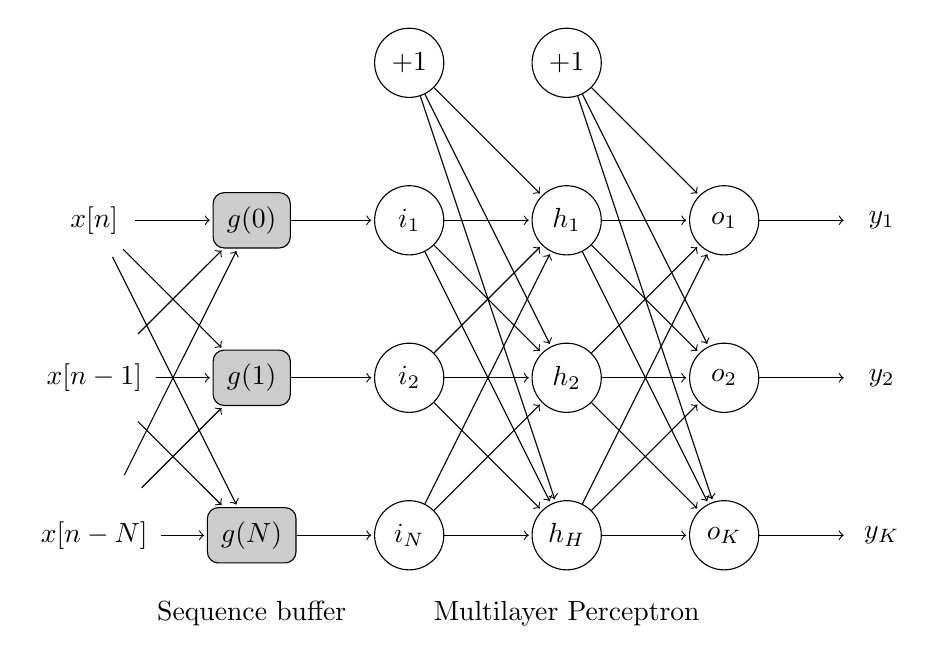
\begin{tikzpicture}[shorten >=1pt,on grid,auto,node distance=2cm] 
   \node[state] (x0)  [draw=none]  {$x[n]$}; 
   \node[state] (x1)   [draw=none,below=of x0] {$x[n-1]$}; 
   \node[state] (xN)   [draw=none,below=of x1] {$x[n-N]$}; 
   \node[fill=black!20,rounded corners, inner sep=5pt, draw] (g0)   [right=of x0] {$g(0)$}; 
   \node[fill=black!20,rounded corners, inner sep=5pt, draw] (g1)   [right=of x1] {$g(1)$}; 
   \node[fill=black!20,rounded corners, inner sep=5pt, draw] (gN)   [right=of xN] {$g(N)$}; 
   \node[] ()   [below=of gN, yshift=1cm] {Sequence buffer}; 
   \node[state] (i1)   [right=of g0] {$i_1$}; 
   \node[state] (ione)   [above=of i1] {+1}; 
   \node[state] (i2)   [below=of i1] {$i_2$}; 
   \node[state] (iN)   [below=of i2] {$i_N$}; 
   \node[state] (hone)   [right=of ione] {+1}; 
   \node[state] (h1)   [below=of hone] {$h_1$}; 
   \node[state] (h2)   [below=of h1] {$h_2$}; 
   \node[state] (hH)   [below=of h2] {$h_H$}; 
   \node[] ()   [below=of hH, yshift=1cm] {Multilayer Perceptron}; 
   \node[state] (o1)   [right=of h1] {$o_1$}; 
   \node[state] (o2)   [below=of o1] {$o_2$}; 
   \node[state] (oK)   [below=of o2] {$o_K$}; 
   \node[state] (y1)   [draw=none,right=of o1] {$y_1$}; 
   \node[state] (y2)   [draw=none,below=of y1] {$y_2$}; 
   \node[state] (yK)   [draw=none,below=of y2] {$y_K$}; 
   \path[->] 
        (x0) edge node {} (g0)
        (x1) edge node {} (g0)
        (xN) edge node {} (g0)
        (x0) edge node {} (g1)
        (x1) edge node {} (g1)
        (xN) edge node {} (g1)
        (x0) edge node {} (gN)
        (x1) edge node {} (gN)
        (xN) edge node {} (gN)
        (g0) edge node {} (i1)
        (g1) edge node {} (i2)
        (gN) edge node {} (iN)
        (ione) edge node {} (h1)
        (ione) edge node {} (h2)
        (ione) edge node {} (hH)
        (i1) edge node {} (h1)
        (i1) edge node {} (h2)
        (i1) edge node {} (hH)
        (i2) edge node {} (h1)
        (i2) edge node {} (h2)
        (i2) edge node {} (hH)
        (iN) edge node {} (h1)
        (iN) edge node {} (h2)
        (iN) edge node {} (hH)
        (hone) edge node {} (o1)
        (hone) edge node {} (o2)
        (hone) edge node {} (oK)
        (h1) edge node {} (o1)
        (h1) edge node {} (o2)
        (h1) edge node {} (oK)
        (h2) edge node {} (o1)
        (h2) edge node {} (o2)
        (h2) edge node {} (oK)
        (hH) edge node {} (o1)
        (hH) edge node {} (o2)
        (hH) edge node {} (oK)
        (o1) edge node {} (y1)
        (o2) edge node {} (y2)
        (oK) edge node {} (yK)
        ;
\end{tikzpicture}
\caption{Time-Delay Neural Network}
\end{figure*}


\begin{figure*}[!h]\centering % Using \begin{figure*} makes the figure take up the entire width of the page
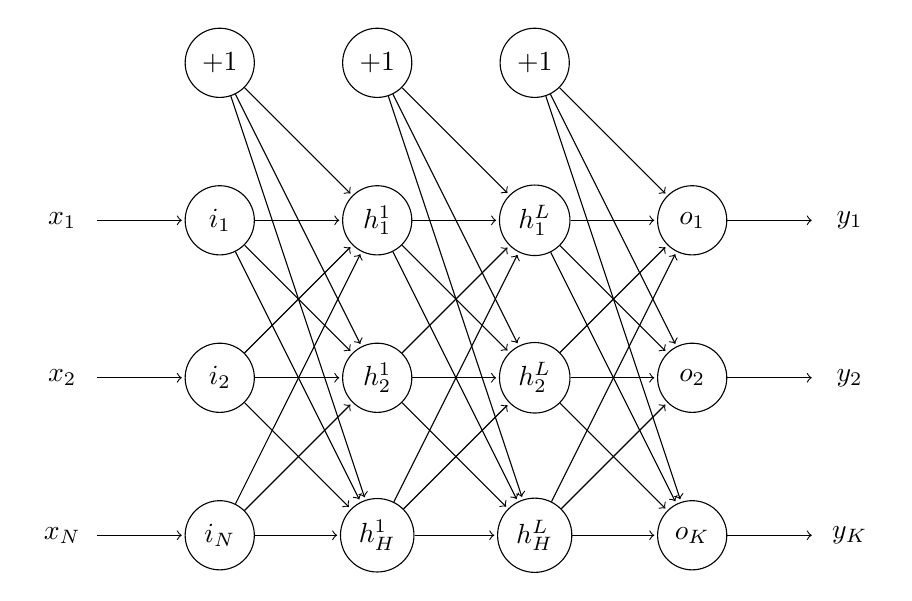
\begin{tikzpicture}[shorten >=1pt,on grid,auto,node distance=2cm] 
   \node[state] (x1)  [draw=none]  {$x_1$}; 
   \node[state] (x2)   [draw=none,below=of x1] {$x_2$}; 
   \node[state] (xN)   [draw=none,below=of x2] {$x_N$}; 
   \node[state] (i1)   [right=of x1] {$i_1$}; 
   \node[state] (ione)   [above=of i1] {+1}; 
   \node[state] (i2)   [below=of i1] {$i_2$}; 
   \node[state] (iN)   [below=of i2] {$i_N$}; 
   \node[state] (hone1)   [right=of ione] {+1}; 
   \node[state] (h11)   [below=of hone1] {$h_1^1$}; 
   \node[state] (h21)   [below=of h11] {$h_2^1$}; 
   \node[state] (hH1)   [below=of h21] {$h_H^1$}; 
   \node[state] (honeL)   [right=of hone1] {+1}; 
   \node[state] (h1L)   [below=of honeL] {$h_1^L$}; 
   \node[state] (h2L)   [below=of h1L] {$h_2^L$}; 
   \node[state] (hHL)   [below=of h2L] {$h_H^L$}; 
   \node[state] (o1)   [right=of h1L] {$o_1$}; 
   \node[state] (o2)   [below=of o1] {$o_2$}; 
   \node[state] (oK)   [below=of o2] {$o_K$}; 
   \node[state] (y1)   [draw=none,right=of o1] {$y_1$}; 
   \node[state] (y2)   [draw=none,below=of y1] {$y_2$}; 
   \node[state] (yK)   [draw=none,below=of y2] {$y_K$}; 
   \path[->] 
        (x1) edge node {} (i1)
        (x2) edge node {} (i2)
        (xN) edge node {} (iN)
        (ione) edge node {} (h11)
        (ione) edge node {} (h21)
        (ione) edge node {} (hH1)
        (i1) edge node {} (h11)
        (i1) edge node {} (h21)
        (i1) edge node {} (hH1)
        (i2) edge node {} (h11)
        (i2) edge node {} (h21)
        (i2) edge node {} (hH1)
        (iN) edge node {} (h11)
        (iN) edge node {} (h21)
        (iN) edge node {} (hH1)

        (hone1) edge node {} (h1L)
        (hone1) edge node {} (h2L)
        (hone1) edge node {} (hHL)
        (h11) edge node {} (h1L)
        (h11) edge node {} (h2L)
        (h11) edge node {} (hHL)
        (h21) edge node {} (h1L)
        (h21) edge node {} (h2L)
        (h21) edge node {} (hHL)
        (hH1) edge node {} (h1L)
        (hH1) edge node {} (h2L)
        (hH1) edge node {} (hHL)
 
        (honeL) edge node {} (o1)
        (honeL) edge node {} (o2)
        (honeL) edge node {} (oK)
        (h1L) edge node {} (o1)
        (h1L) edge node {} (o2)
        (h1L) edge node {} (oK)
        (h2L) edge node {} (o1)
        (h2L) edge node {} (o2)
        (h2L) edge node {} (oK)
        (hHL) edge node {} (o1)
        (hHL) edge node {} (o2)
        (hHL) edge node {} (oK)
        (o1) edge node {} (y1)
        (o2) edge node {} (y2)
        (oK) edge node {} (yK)
        ;
\end{tikzpicture}
\caption{Deep Learning network}
\end{figure*}


\begin{figure*}[!h]\centering % Using \begin{figure*} makes the figure take up the entire width of the page
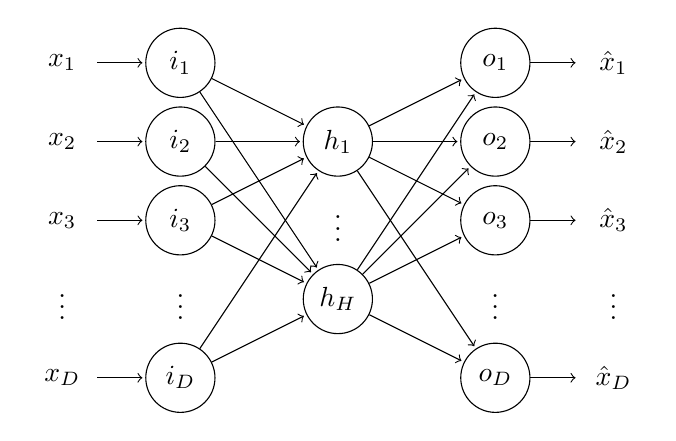
\begin{tikzpicture}[shorten >=1pt,on grid,auto,node distance=1.0cm]
   \node[state] (x1)  [draw=none]  {$x_1$}; 
   \node[state] (x2)   [draw=none,below=of x1] {$x_2$}; 
   \node[state] (x3)   [draw=none,below=of x2] {$x_3$}; 
   \node[state] (xdots)   [draw=none,below=of x3] {$\vdots$}; 
   \node[state] (xD)   [draw=none,below=of xdots] {$x_D$}; 
   \node[state, node distance=1.5cm] (i1)   [right=of x1] {$i_1$}; 
   \node[state] (i2)   [below=of i1] {$i_2$}; 
   \node[state] (i3)   [below=of i2] {$i_3$}; 
   \node[state] (idots)   [draw=none,below=of i3] {$\vdots$}; 
   \node[state] (iD)   [below=of idots] {$i_D$}; 
   \node[state, node distance=2cm] (h1)   [right=of i2] {$h_1$}; 
   \node[state] (hdots)   [draw=none,below=of h1] {$\vdots$}; 
   \node[state] (hH)   [below=of hdots] {$h_{H}$}; 
   \node[state, node distance=2cm] (o2)   [right=of h1] {$o_2$}; 
   \node[state] (o1)   [above=of o2] {$o_1$}; 
   \node[state] (o3)   [below=of o2] {$o_3$}; 
   \node[state] (odots)   [draw=none,below=of o3] {$\vdots$}; 
   \node[state] (oD)   [below=of odots] {$o_D$}; 
   \node[state, node distance=1.5cm] (xx1) [draw=none,right=of o1] {$\hat{x}_1$};
   \node[state] (xx2)   [draw=none,below=of xx1] {$\hat{x}_2$}; 
   \node[state] (xx3)   [draw=none,below=of xx2] {$\hat{x}_3$}; 
   \node[state] (xxdots)   [draw=none,below=of xx3] {$\vdots$}; 
   \node[state] (xxD)   [draw=none,below=of xxdots] {$\hat{x}_D$}; 
   \path[->] 
        (x1) edge node {} (i1)
        (x2) edge node {} (i2)
        (x3) edge node {} (i3)
        (xD) edge node {} (iD)
        (i1) edge node {} (h1)
        (i1) edge node {} (hH)
        (i2) edge node {} (h1)
        (i2) edge node {} (hH)
        (i3) edge node {} (h1)
        (i3) edge node {} (hH)
        (iD) edge node {} (h1)
        (iD) edge node {} (hH)
        (h1) edge node {} (o1)
        (h1) edge node {} (o2)
        (h1) edge node {} (o3)
        (h1) edge node {} (oD)
        (hH) edge node {} (o1)
        (hH) edge node {} (o2)
        (hH) edge node {} (o3)
        (hH) edge node {} (oD)
        (o1) edge node {} (xx1)
        (o2) edge node {} (xx2)
        (o3) edge node {} (xx3)
        (oD) edge node {} (xxD)
        ;

%\begin{pgfonlayer}{background}
%    \filldraw [line width=6mm,join=round,black!10]
%      (ione.north -| ione.west) rectangle (i4.south -| o1.east);
%\end{pgfonlayer}

\end{tikzpicture}
\caption{Auto-encoder}
\end{figure}


\end{document}
